\subsubsection{Verkehrsaufkommen}
\label{sec:traffic_volume_definition}

\paragraph{[FR3]} \textit{NUNAV Navigation} muss den \textit{End Usern} während der Navigation Informationen zum Verkehrsgeschehen auf der aktuellen Route liefern.

Wie aus der Persona von Michael hervorgeht, wundert er sich zum Teil, warum \textit{NUNAV Navigation} aus seiner Sicht \glqq komische\grqq{} Routen vorschlägt. Ein Erklärungsansatz ist, das Verkehrsgeschehen auf der aktuellen Route anzuzeigen. Diese \textit{Context}-Information soll dabei helfen zu verstehen, warum \textit{NUNAV Navigation} andere Routen wählt. 

Dies ist allerdings nicht trivial, da die Berechnung des Verkehrsaufkommens und dessen subjektive Warhnehmung der \textit{End User} nicht klar ist. Ein weiteres Problem ist, dass es nicht möglich ist, zu berechnen, welche Route für Nutzer auf der gleichen Strecke subjektiv als \glqq normal\grqq{} empfunden wird. Nachdem mehrere Lösungsansätze für dieses Problem in kleinen Runden bei Graphmasters diskutiert wurden, wird als Lösung die Berechnung des Verhältnisses von durchschnittlicher Dauer der Route zu aktueller Dauer als Basiswert genommen. Die Daten werden dabei durch \textit{Nugraph} zur Verfügung gestellt und im Rahmen dieser Arbeit im \textit{BFF} auf die Stufen \glqq wenig Verkehr\grqq{}, \glqq mäßiger Verkehr\grqq{} und \glqq viel Verkehr\grqq{} abgebildet. Außerdem gibt es eine \glqq normale\grqq{} Verkehrssituation, in der den \textit{End Usern} keine Erklärung angezeigt wird. Die Abbildungsfunktion ist in den Zusatzmaterialien zu finden. Die Schwellwerte wurden intern durch Testfahrten ermittelt.

Die Informationen können \textit{End User} auf drei Wegen erhalten. Zunächst werden die Informationen in der Routenvorschau angezeigt. Dabei wird die Gesamtfahrzeit für die Route je nach Verkehrsaufkommen grün (wenig Verkehr), Standardtextfarbe (normaler Verkehr), orange (mäßiger Verkehr) und rot (viel Verkehr) dargestellt. Da im ersten Prototypen aufgefallen ist, dass die Farben alleine nicht aussagekräftig sind (siehe \autoref{fig:prototype_traffic_volume_route}, (a)), wurde zusätzlich ein kurzer Erklärungstext eingefügt (siehe \autoref{fig:prototype_traffic_volume_route}, (b)). Dieser ist bei \glqq normalem\grqq{} nicht zu sehen. So lernen die \textit{End User} mit der Zeit die Bedeutung der Farben. Eine Übersicht mit allen Prototypen ist in \nameref{ch:appendix_1} zu finden.

Außerdem werden während der gesamten Navigation die Ankunftszeit und die Fahrzeit in der entsprechenden Farbe angezeigt und bei sich ändernder Verkehrssituation auch aktualisiert.

\begin{figure}[htb!]
    \centering
    \subfloat[Prototyp zur Darstellung des aktuellen Verkehrsaufkommens in der Routenvorschau]
    {
        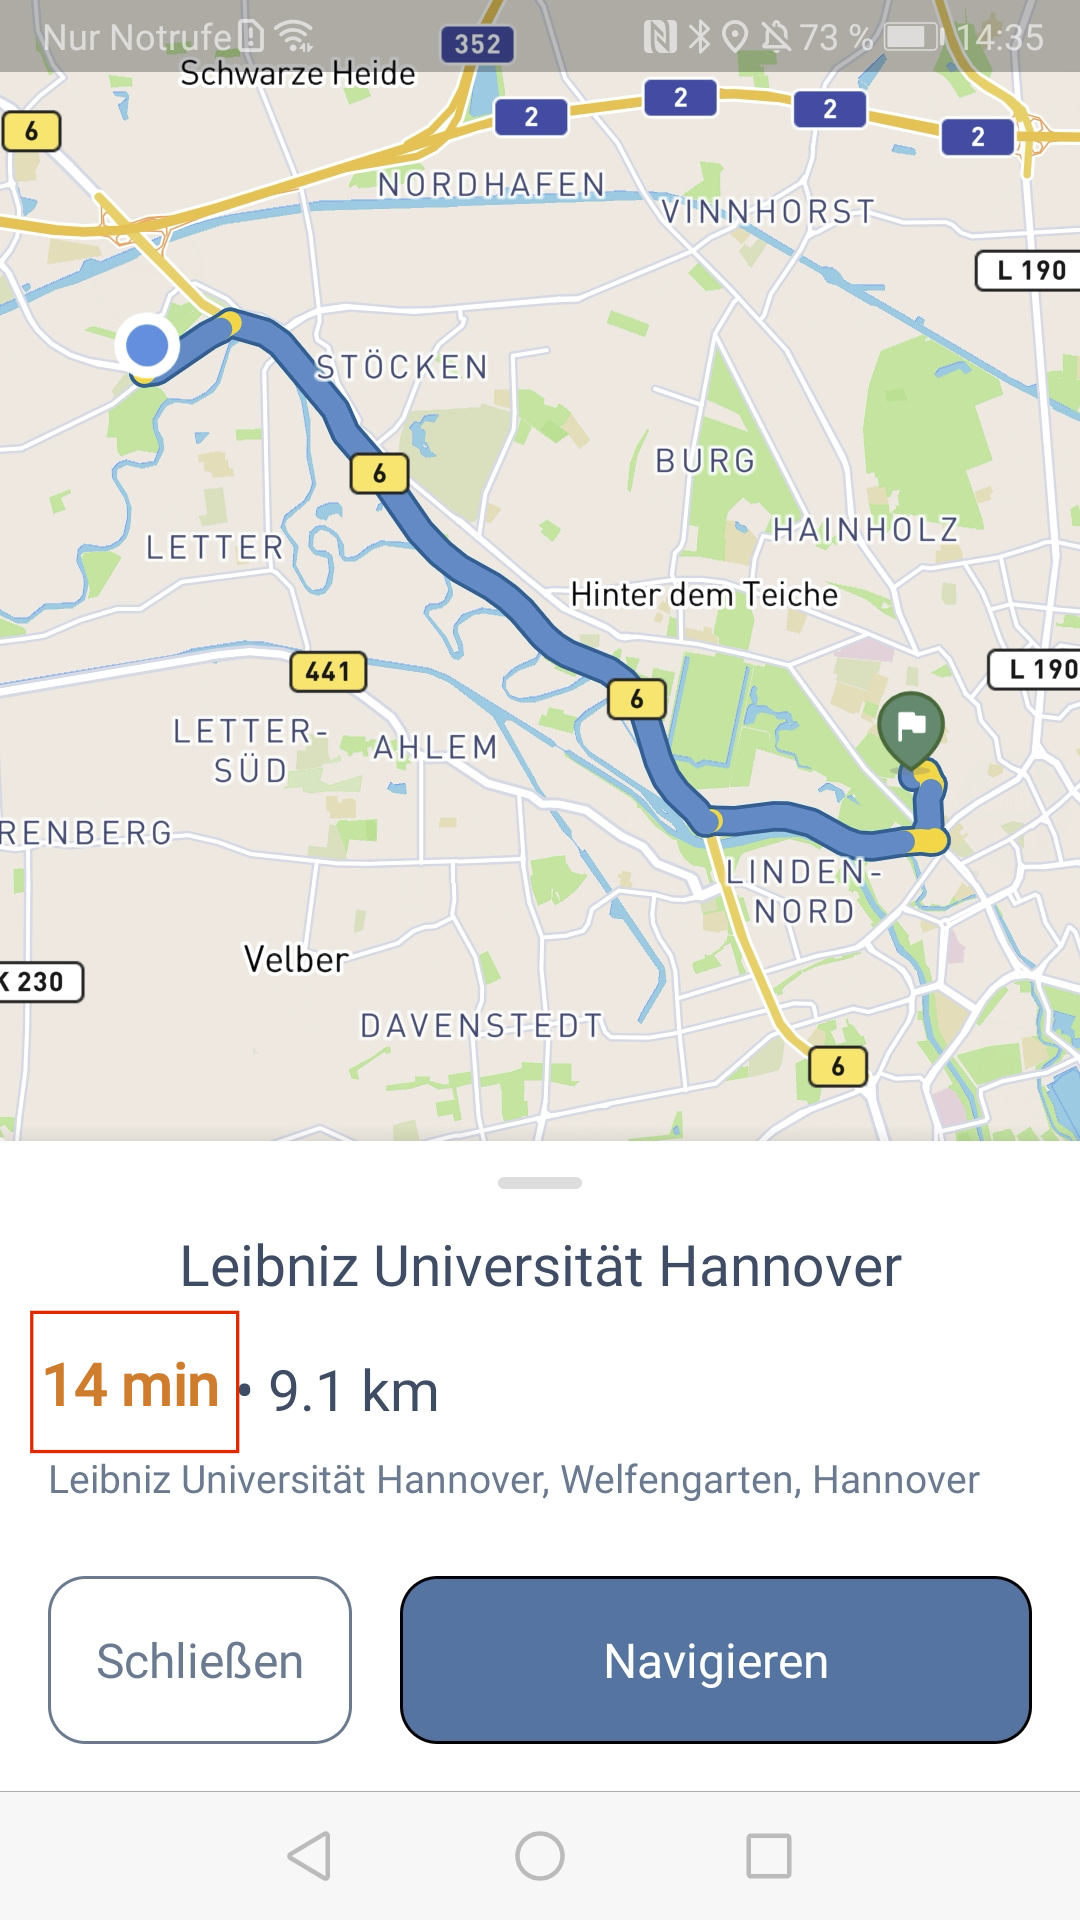
\includegraphics[width=.27\textwidth]{contents/06_model_evaluation/01_integration/res/03_traffic_volume/prototype_11.png}
    }
    \hspace{.055\textwidth}
    \subfloat[Finales Design zur Darstellung des aktuellen Verkehrsaufkommens in der Routenvorschau]
    {
        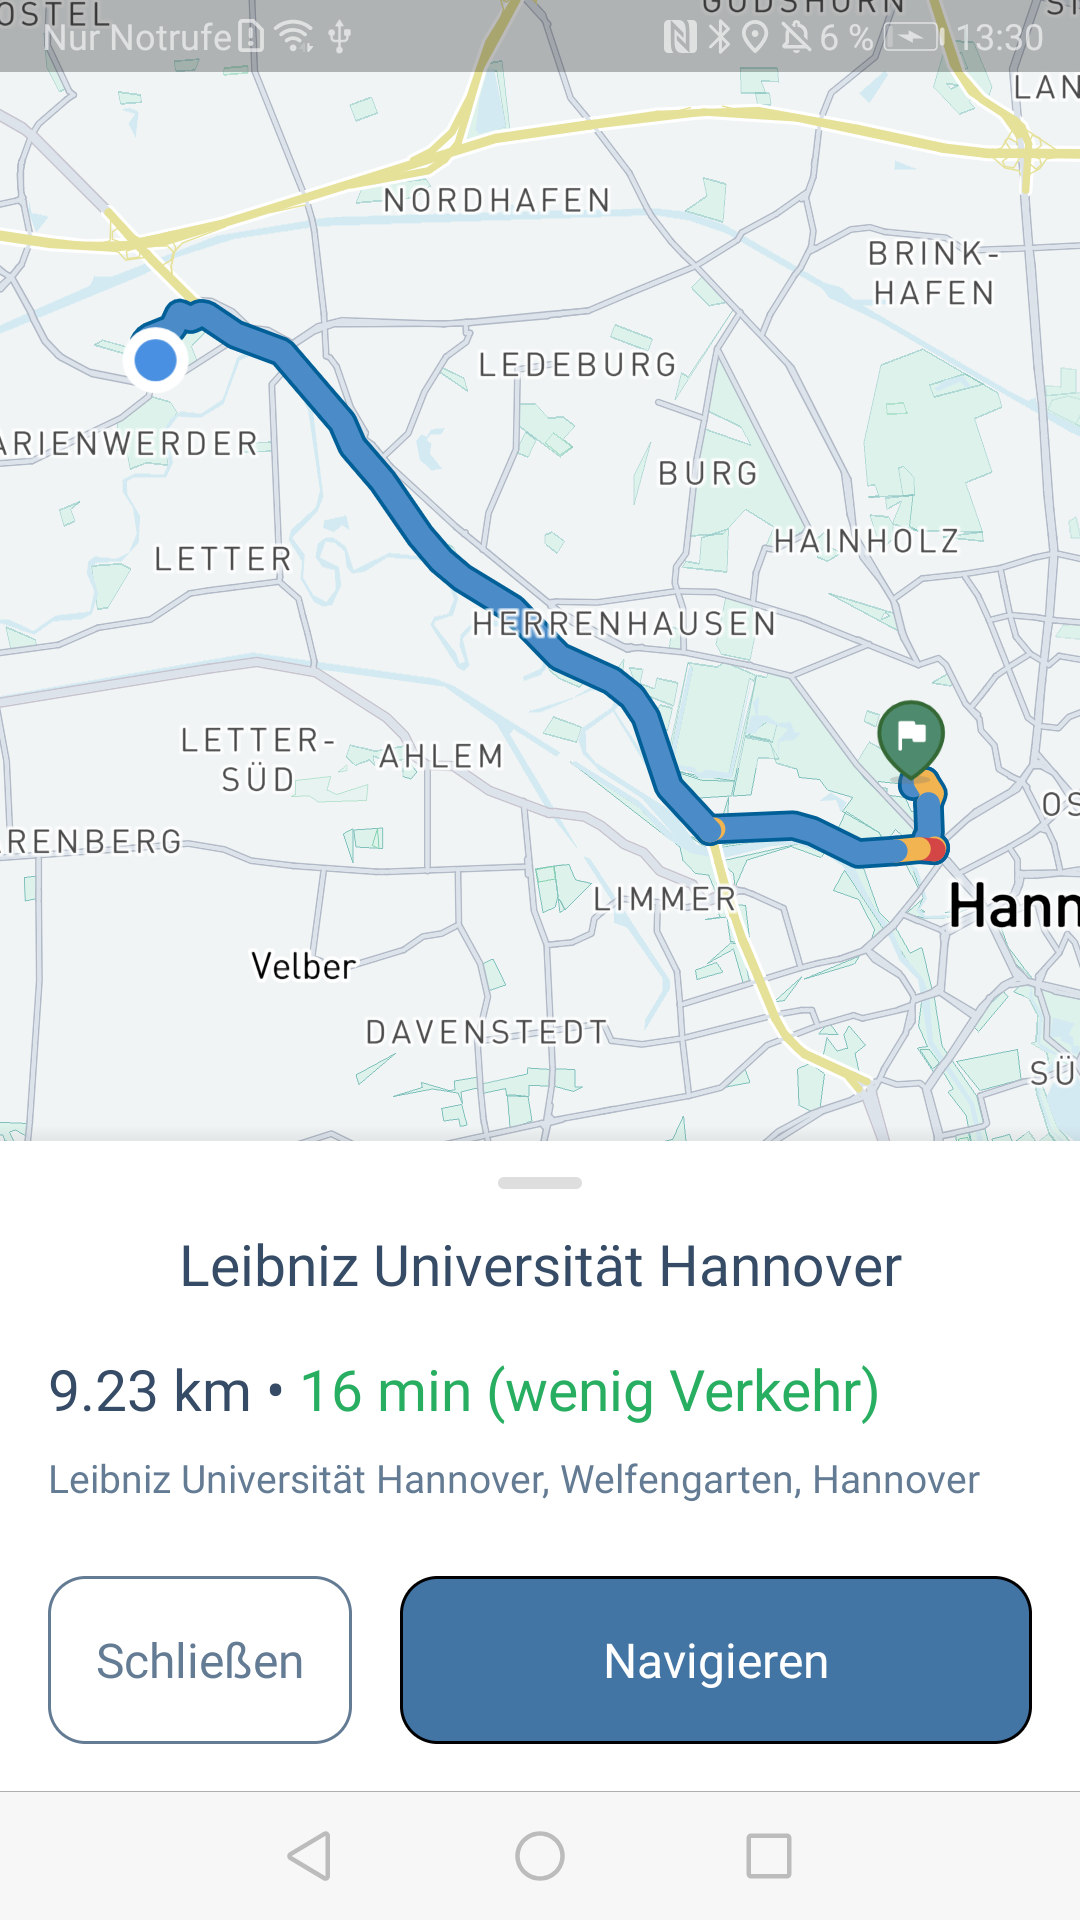
\includegraphics[width=.27\textwidth]{contents/06_model_evaluation/01_integration/res/03_traffic_volume/final_10.png}
    }
    \hspace{.055\textwidth}
    \subfloat[Finales Design zur Darstellung des aktuellen Verkehrsaufkommens während der Navigation]
    {
        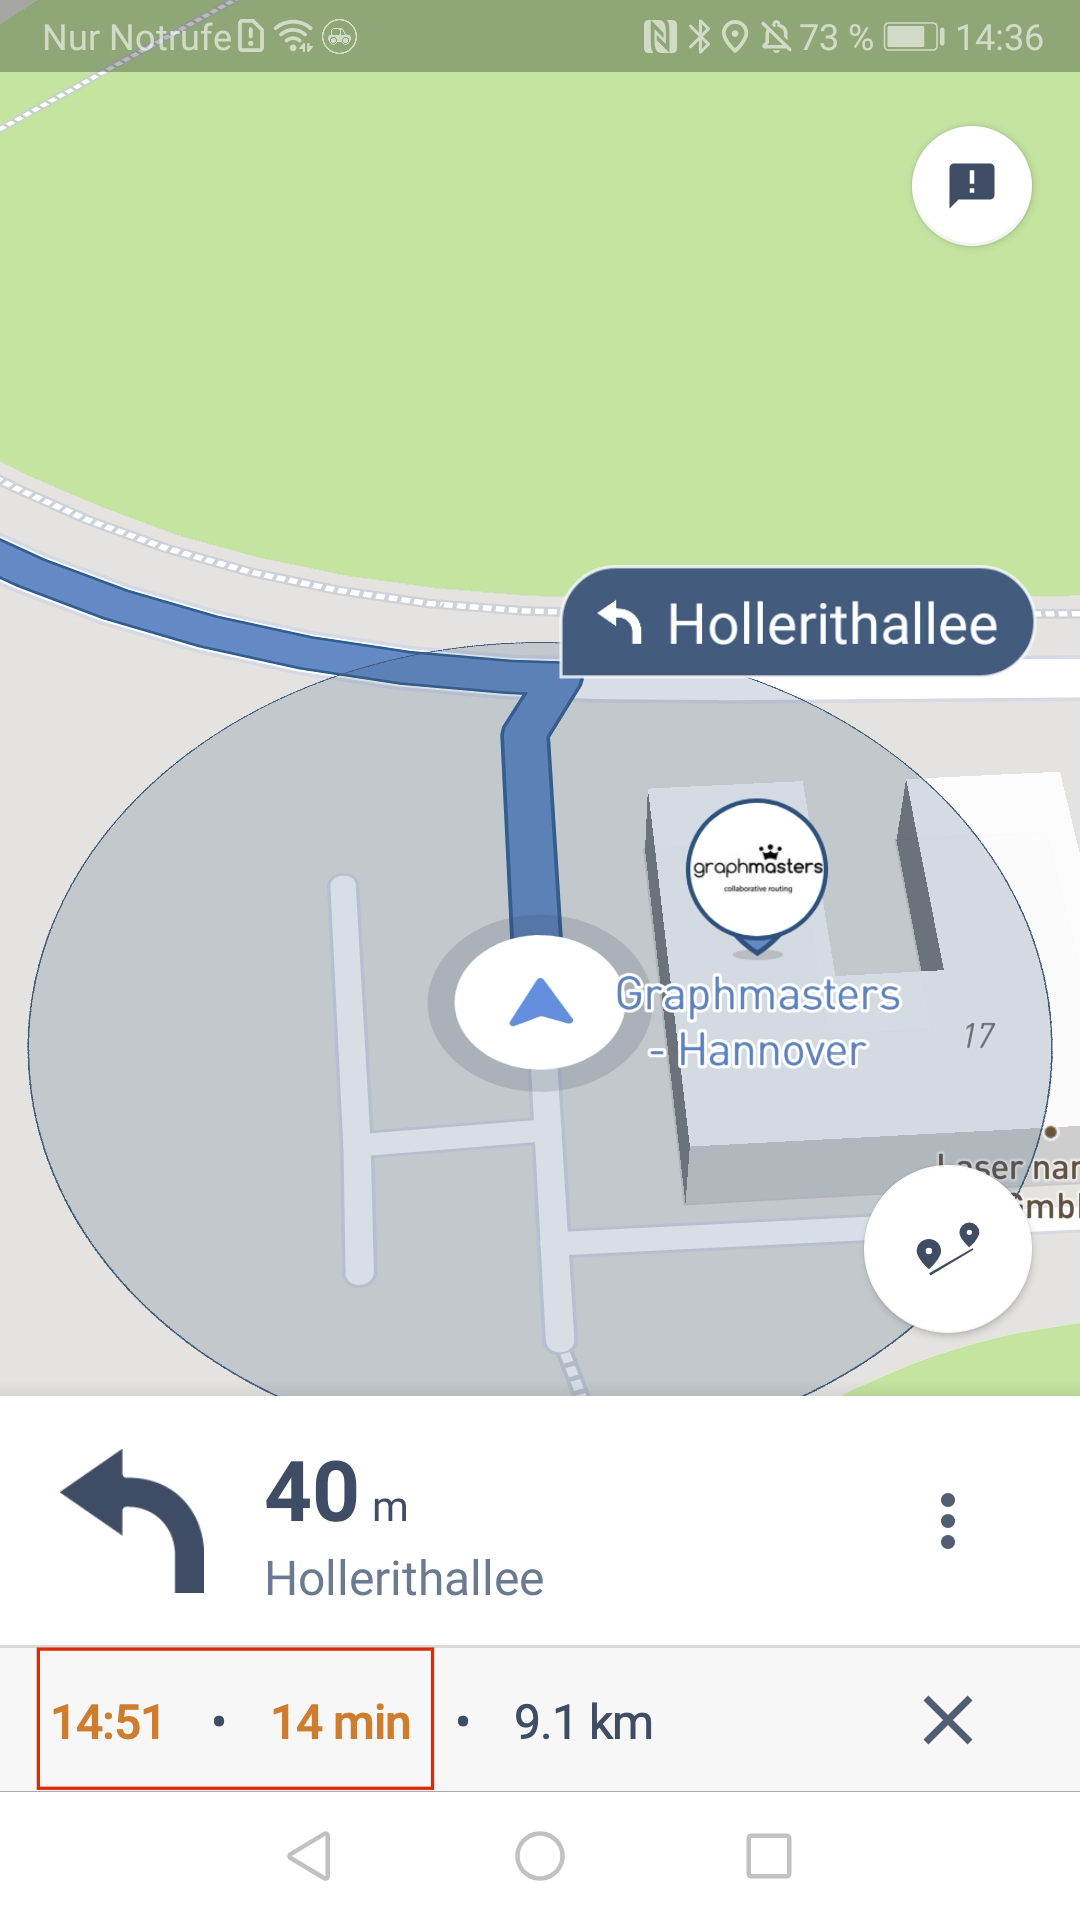
\includegraphics[width=.27\textwidth]{contents/06_model_evaluation/01_integration/res/03_traffic_volume/final_20.png}
    }
    \caption{Prototyp und finale Designs für die Erklärung zum kollaborativem Routing}
    \label{fig:prototype_traffic_volume_route}
\end{figure}

Des Weiteren ist das Sprachkommando, welches bei Start der Navigation gegeben wird, je nach Verkehrssituation unterschiedlich (siehe \autoref{tab:voice_commands_traffic_volume}).

\begin{table}[bht!]
    \begin{tabular}{p{.25\textwidth}p{.71\textwidth}}
        \hline
        Verkehrsaufkommen        & Sprachkommando \\
        \toprule
        wenig & Heute sind die Straßen frei. Du wirst dein Ziel <Zielname> um <Uhrzeit> erreichen. \\
        \tablerowspacing
        normal & Du wirst dein Ziel <Zielname> um <Uhrzeit> erreichen. \\
        \tablerowspacing
        mäßig & Da heute etwas mehr los ist, wirst du dein Ziel <Zielname> um <Uhrzeit> erreichen. \\
        \tablerowspacing
        viel & Da heute sehr viel los ist, wirst du dein Ziel <Zielname> um <Uhrzeit> erreichen. \\
        \toprule
    \end{tabular}
\caption{Sprachkommandos zum Start der Navigation abhängig von der Verkehrssituation}
\label{tab:voice_commands_traffic_volume}
\end{table}